\section{Tuesday, 23 October 2018}

\subsection{Steps}
\begin{itemize}
\item We have studied the operation of clustering algorithm to identify outliers, which is DBSCAN
\item We have based in the moodle example and we have tried to do \texttt{DBSCAN}  with a symetric matrix  but we didn't understand the results.
\item Then we decided to use a conectivity matrix as input for a hierarchical clustering algorithm (\texttt{AgglomerativeClustering}). This conectivity matrix was obtained applying the \textit{``k nearest neighbors''}  algorithm. This algorithm returns a matrix that indicates what $k$ neighbors is connected an element from the matrix \texttt{AgglomerativeClustering} returns a clusters hierarchy.

\begin{figure}[!htb]
\centering
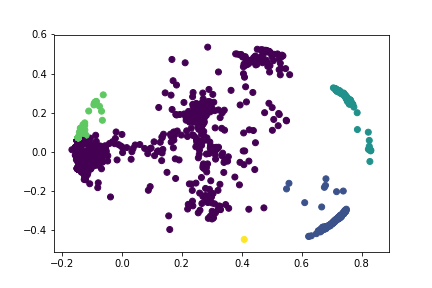
\includegraphics[width=0.5\textwidth]{../../reports/figures/AgglomerativeClustering_AccelerometerStat.png}
\caption{Agglomerative Clustering algorithm using a knn conectivity matrix}
\label{fig:agglomerative}
\end{figure}

\item We have applied the \texttt{DBSCAN} algorithm to know what points from the dataset are core points, what points are border points and which ones are noise. The noise points will be considered outliers.

\item We have plotted the \texttt{DBSCAN} graphics to see the outliers.

\begin{figure}[!htb]
\centering
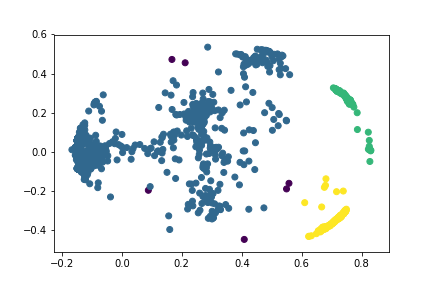
\includegraphics[width=0.5\textwidth]{../../reports/figures/DBSCAN_AccelerometerStat.png}
\caption{DBSCAN algorithm, used to identify outliers}
\label{fig:dbscan}
\end{figure}

\end{itemize}